\documentclass[10pt]{standalone}
\usepackage[utf8]{inputenc}
\usepackage{pgf,tikz,pgfplots}
\pgfplotsset{compat=1.15}
\usepackage{mathrsfs}
\usetikzlibrary{arrows}
\pagestyle{empty}

\begin{document}

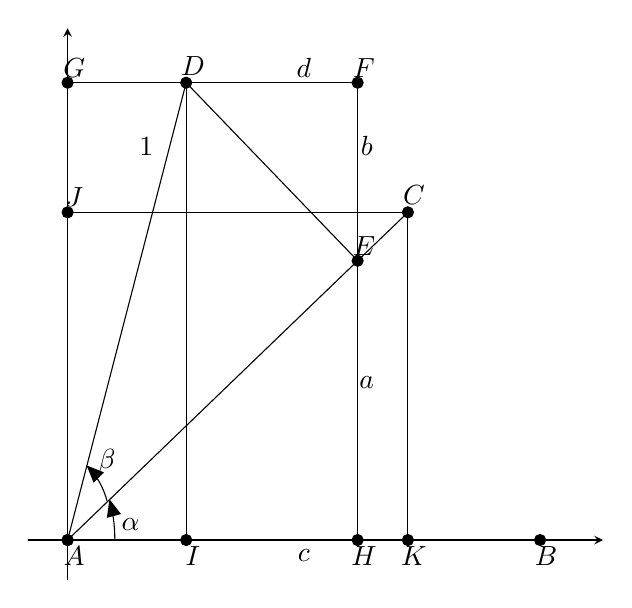
\begin{tikzpicture}[line cap=round,line join=round,>=triangle 45,x=1.0cm,y=1.0cm]
\begin{axis}[
x=1.0cm,y=1.0cm,
axis lines=middle,
xmin=-0.5,
xmax=6.8,
ymin=-0.5,
ymax=6.5,
ticks=none,]
\clip(-0.5,-0.5) rectangle (6.8,6.5);

\draw  (0.,0.)-- (6.,0.);
\draw  (0.,0.)-- (4.321792159980355,4.161984205391983);
\draw  (0.,0.)-- (1.5060222368775498,5.807916754054792);
\draw  (1.5060222368775498,5.807916754054792)-- (3.6832681240743588,3.547071027286727);
\draw  (0.,5.807916754054792)-- (3.683268124074359,5.807916754054791);
\draw  (3.683268124074359,5.807916754054791)-- (3.6832681240743588,0.);
\draw  (1.5060222368775495,0.)-- (1.5060222368775498,5.807916754054792);
\draw  (0.,4.161984205391983)-- (4.321792159980355,4.161984205391983);
\draw  (4.321792159980355,4.161984205391983)-- (4.321792159980355,0.);
\begin{scriptsize}
\draw  (0 ,0) circle [radius=2.0pt];
\draw (0.08331531988857643,-0.2) node {$A$};
\draw[->] (0.6,0) arc (0:15:2cm);
\draw (0.8,0.2) node {$\alpha$};
\draw[->] (0.5,.5) arc (15:45:1cm);
\draw (0.5,1.0) node {$\beta$};
\draw (3.8 ,2) node {$a$};
\draw (3.8 ,5) node {$b$};
\draw [fill=black] (6.,0.) circle[radius=2.0pt];
\draw [fill=black] (0.,0.) circle[radius=2.0pt];
\draw (6.077730011761241,-0.2) node {$B$};
\draw (3.0,-0.2) node {$c$};
\draw (3.0,6) node {$d$};
\draw (1.0,5) node {$1$};
\draw [fill=black] (4.321792159980355,4.161984205391983) circle [radius=2.0pt];
\draw (4.397913226706713,4.377852695182037) node {$C$};
\draw [fill=black] (1.5060222368775498,5.807916754054792) circle [radius=2.0pt];
\draw (1.5905481886703787,6.023152696982021) node {$D$};
%\draw (0.9577404956703854,2.9626645817456874) node {$h$};
\draw [fill=black] (3.6832681240743588,3.547071027286727) circle [radius=2.0pt];
\draw (3.76510553370672,3.7335394077638617) node {$E$};
%\draw (2.4879845532885514,4.653986961218398) node {$j$};
\draw [fill=black] (3.683268124074359,5.807916754054791) circle [radius=2.0pt];
\draw (3.76510553370672,6.000141508145657) node {$F$};
\draw [fill=black] (0.,5.807916754054792) circle [radius=2.0pt];
\draw (0.08331531988857643,6.000141508145657) node {$G$};
\draw [fill=black] (3.6832681240743588,0.) circle [radius=2.0pt];
\draw (3.76510553370672,-0.2) node {$H$};
\draw [fill=black] (1.5060222368775495,0.) circle [radius=2.0pt];
\draw (1.5905481886703787,-0.2) node {$I$};
%\draw (1.8666824547067395,5.7240072421092965) node {$n$};
%\draw (3.5234880509249042,3.008686959418414) node {$p$};
%\draw (1.7171097272703775,3.008686959418414) node {$q$};

\draw [fill=black] (0.,4.161984205391983) circle [radius=2.0pt];
\draw (0.08331531988857643,4.354841506345673) node {$J$};
\draw [fill=black] (4.321792159980355,0.) circle [radius=2.0pt];
\draw (4.397913226706713,-0.2) node {$K$};
%\draw (2.1888390984158272,4.0787072403093125) node {$t$};
%\draw (4.167801338343079,2.180284161309331) node {$a$};
\end{scriptsize}
\end{axis}
\end{tikzpicture}
\end{document}